% 复环面：格 Lambda 与基本平行四边形
\documentclass[border=4pt]{standalone}
\usepackage{tikz}
\usetikzlibrary{arrows.meta}
\usepackage{amsmath,amssymb}
\definecolor{fillA}{rgb}{0.45,0.45,0.45}
\definecolor{fillB}{rgb}{0.72,0.72,0.72}
\begin{document}
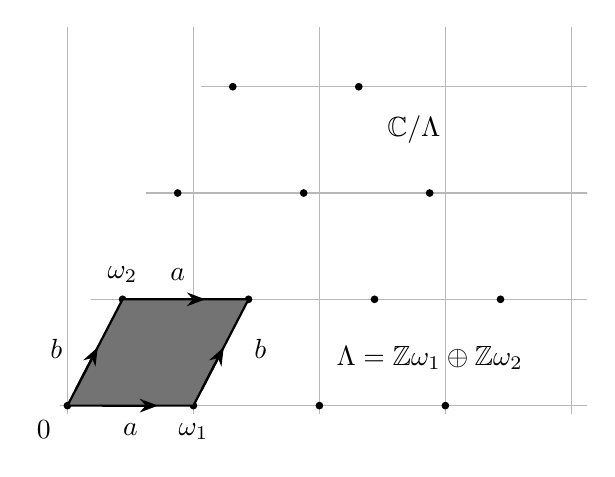
\begin{tikzpicture}[>=Stealth, line cap=round]
% 格点网
\begin{scope}
  \clip (-0.1,-0.1) rectangle (6.6,4.8);
  \foreach \n in {-1,0,1,2,3}
    \draw[fillB, thin] (\n*0.7-0.4, \n*1.35) -- (\n*0.7+6.6, \n*1.35);
  \foreach \m in {-1,0,1,2,3,4}
    \draw[fillB, thin] (\m*1.6, -0.4) -- (\m*1.6, 5.0);
\end{scope}
% 格点
\foreach \p in {(0,0),(1.6,0),(3.2,0),(4.8,0),(0.7,1.35),(2.3,1.35),(3.9,1.35),(5.5,1.35),(1.4,2.7),(3.0,2.7),(4.6,2.7),(2.1,4.05),(3.7,4.05)}
  \fill \p circle (1.4pt);
% 基本平行四边形
\fill[fillA] (0,0) -- (1.6,0) -- (2.3,1.35) -- (0.7,1.35) -- cycle;
\draw[thick] (0,0) -- (1.6,0) -- (2.3,1.35) -- (0.7,1.35) -- cycle;
% 对边粘合（箭头同向）
\draw[->, thick] (0.45,0) -- (1.15,0);
\draw[->, thick] (1.05,1.35) -- (1.75,1.35);
\draw[->, thick] (0.105,0.2025) -- (0.385,0.7425);
\draw[->, thick] (1.705,0.2025) -- (1.985,0.7425);
\node at (0.8,-0.3) {$a$};
\node at (1.4,1.66) {$a$};
\node at (-0.14,0.72) {$b$};
\node at (2.45,0.72) {$b$};
% 标注
\node at (-0.3,-0.3) {$0$};
\node at (1.6,-0.33) {$\omega_1$};
\node at (0.7,1.66) {$\omega_2$};
\node at (4.4,3.5) {$\mathbb C/\Lambda$};
\node at (4.6,0.6) {$\Lambda=\mathbb Z\omega_1\oplus\mathbb Z\omega_2$};
\end{tikzpicture}
\end{document}
